\documentclass{article}
\usepackage{geometry}
\usepackage{flafter}
\geometry{letterpaper, portrait, margin=1in}

\usepackage{hyperref}
\hypersetup{
    colorlinks=true,
    linkcolor=black,
    filecolor=magenta,
    urlcolor=blue,
}

\usepackage{graphicx}
\graphicspath{ {images/} }

\usepackage{tcolorbox}
\usepackage{textcomp}
\usepackage{gensymb}
\usepackage{indentfirst}

\newcommand{\ans}{$\rule{1.5cm}{0.15mm}$}

\title{RoboJackets Electrical Training Week 0 Worksheet}
\author{Alex Xu \\ Joe Spall}
\date{\today\\v1.1}

\begin{document}
\maketitle{}
\setcounter{tocdepth}{2}
\tableofcontents
\pagebreak

\section{What is this worksheet? What's so special about it? Why should you read it?}
There are three documents in the Week 0 training: a worksheet, its answer sheet and an informational sheet that explains everything in this document. This document is the worksheet.
\vspace{6pt}\par
RoboJackets build robots, and we are going to help you understand how we built them so you can do it as well. The electrical training focuses on the idea of ``Prototyping", which requires a basic understanding of electricity. We therefore prepared Week 0 session for those have little knowledge in electricity so you'll walk in to Week 1 less confused. \vspace{6pt}\par
This worksheet contains all \textbf{a variety questions pertaining to information you should know when you walk into Week 1} electrical training session. It is perfectly fine if you do not know certain, or any, concepts covered in this worksheet. If there are any concepts in this worksheet you do not feel comfortable with, please ask any of the instructors or your classmates for help. For more background on the topics, you can also refer to the Informational Sheet. Please only refer to the Answer Sheet after you have attempted to answer all of the questions.\vspace{6pt}\par

\section{Intro to Electricity}
\begin{enumerate}
	\item Resistance is measured in \ans. (Unit)
	\item If the two terminals of a resistor are measured to be -3.3V and -5V with reference to some arbitrary pre-defined ground. The potential difference across the resistor is \ans.
	\item To measure current,an Ammeter is connected in \ans\ (parallel / series) with the desired path. To measure voltage, a Voltmeter is connected in \ans\ (parallel / series) with the desired path.
	\item 5V is applied across a resistor and the resultant current is 0.2A. The resistance across the resistor is \ans.
	\item The resistor in the previous question is dissipating energy at \ans W.
	\item With reference to the color coding diagram (Figure \ref{fig:Resistor}), a resistor of yellow, violet, brown and gold color code has a resistance of \ans.
	\begin{figure}
		\center
		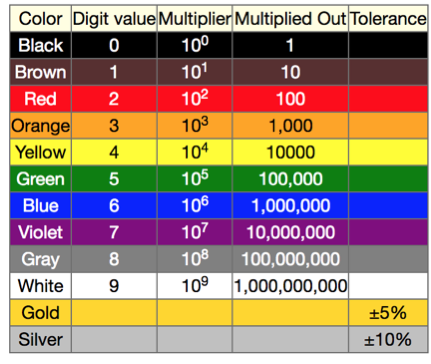
\includegraphics[width=0.4\textwidth, keepaspectratio]{rcolorcoding}
		\caption{Resistor Coding Chart}
		\label{fig:Resistor}
	\end{figure}
\end{enumerate}

\section{Capacitors and Inductors}
\subsection{Capacitors}
\begin{enumerate}
	\item Capacitors are measured in \ans. (Unit)
	\item 0.0025 coulomb of charge accumulates across a capacitor when 5V is applied, its capacitance is \ans.
	\item There are two types of capacitors: ceramic and electrolytic. Both of them do not have polarity (True / False).
	\item Electrolytic capacitors usually have a lower value than ceramic capacitors. (True / False)
	\item Capacitors are used in circuits for what purposes related to power?
\end{enumerate}
\subsection{Inductors}
\begin{enumerate}
	\item Inductors are measured in \ans. (Unit)
	\item Inductors can typically be found in electro-mechanical parts on a robot. (True / False)
	\item An ohmmeter is connected across an inductor and the meter reads zero ohms. The inductor is definitely broken. (True / False)
\end{enumerate}

\section{Diodes and FETs}
\begin{enumerate}
	\item LEDs are a type of diode, and they're very delicate. We need to apply additional resistors in series to an LED to prevent too much current. If the supply voltage is 5V and the LED is rated at 20mA maximum, what's the minimum resistance of the additional resistor?
	\item FETs are used to help low voltage logic circuits to control high voltage and current-drawing motors. (True / False)
	\item For the Figure \ref{fig:transistor}, assume the two transistors are functioning properly with respect to Vdd and Vss levels. What's the voltage level of Q when voltage at A equals Vdd?

	\begin{figure}[!h]
		\center
		
\includegraphics[width=0.2\textwidth, keepaspectratio]{fetoperation}
		\caption{Transistor Operation Schematics}
		\label{fig:transistor}
	\end{figure}
\end{enumerate}
\clearpage
\section{Circuit Analysis}
\subsection{Parallel and Series}
\begin{enumerate}
	\item Two $1.2 k \ohm$ resistors are in series, and this combination is in parallel with a $3.3 k\ohm$ resistor (left circuit in Figure \ref{fig:parallel}). The total resistance is \ans.
	\item Consider the right circuit in Figure \ref{fig:parallel}. Assume ECHO\_5V is actually 5V. What's the voltage at ECHO\_OUT?
	\item A $10 \mu F$, $20 \mu F$, $22 \mu F$, and $100 \mu F$ capacitor are in parallel. The total capacitance is \ans.
	\item Now the capacitors in Q3 are in series. Their capacitance is \ans.
	
	\begin{figure}[h]
		\center
		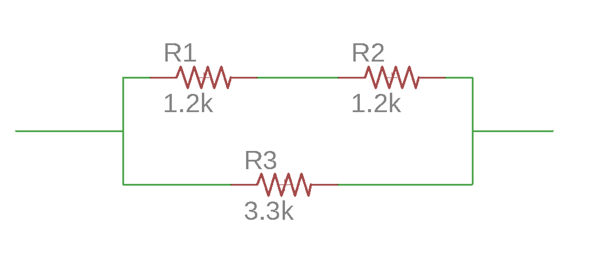
\includegraphics[width=0.5\textwidth, keepaspectratio]{parallel}
		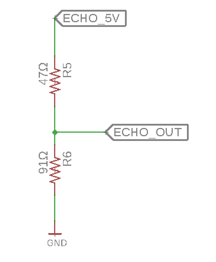
\includegraphics[width=0.2\textwidth, keepaspectratio]{vdivide}
		\caption{Parallel and Series Analysis}
		\label{fig:parallel}
	\end{figure}
	
	
\end{enumerate}
\subsection{Kirchoff's Law}
\begin{enumerate}
	\item In Figure \ref{fig:kirchof}, $R_1=4\ohm ,R_2=3\ohm,R_3=2\ohm, \varepsilon_1=12V, \varepsilon_2=8V$. What's the current through $ R_2 $.
	\begin{figure}[!h]
		\center
		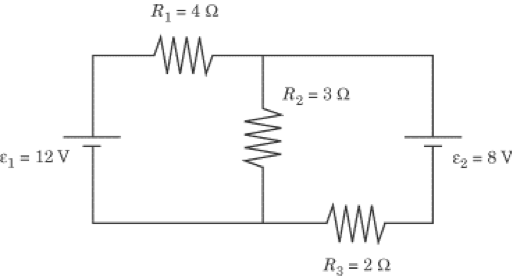
\includegraphics[width=0.4\textwidth, keepaspectratio]{kirchof}
		\caption{Kirchoff's Circuit Analysis}
		\label{fig:kirchof}
	\end{figure}
\end{enumerate}
\clearpage
\section{Prototyping}
\begin{enumerate}
	\item Breadboards are very useful during prototyping. If the breadboard in front of you is oriented so that the longer side faces you (see Figure \ref{fig:bread}). Holes in the same rows are \ans\ and those in the same column are \ans. Columns on the two sides of the middle trench are \ans\ (Fill in with Connected or Not connected). 
	\item When prototyping with breadboard, you should use \ans\ (single-core / multi-core) for a signal line. When crimping a multi-core wire, one (should / should not) twist the wire to make it more solid. 
	\item Is R1 in the right-sided circuit of Figure \ref{fig:bread} acting as a pull-down resistor or pull-up resistor? What does it do?
	\begin{figure}[h]
		\center
		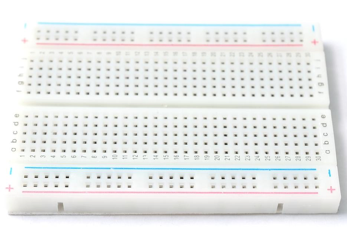
\includegraphics[width=0.27\textwidth, keepaspectratio]{bread}
		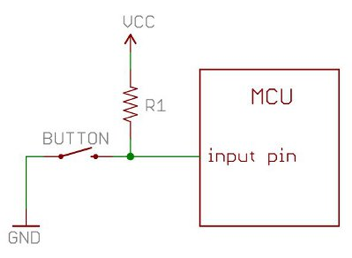
\includegraphics[width=0.27\textwidth, keepaspectratio]{pull}
		\caption{Example breadboard and pull-up resistor network}
		\label{fig:bread}
	\end{figure}
	\item Fuse is the most fragile part of your circuit. Replace it with a wire to make your circuit more robust (True / False).
\end{enumerate}
\end{document}